%% LaTeX-Beamer template for KIT design
%% by Erik Burger, Christian Hammer
%% title picture by Klaus Krogmann
%%
%% version 2.1
%%
%% mostly compatible to KIT corporate design v2.0
%% http://intranet.kit.edu/gestaltungsrichtlinien.php
%%
%% Problems, bugs and comments to
%% burger@kit.edu

\documentclass[18pt]{beamer}

%% SLIDE FORMAT

% use 'beamerthemekit' for standard 4:3 ratio
% for widescreen slides (16:9), use 'beamerthemekitwide'

\usepackage{templates/beamerthemekit}
%\usepackage{templates/beamerthemekitwide}
\usepackage{multirow}

\usepackage{tabularx}
\newcolumntype{R}[1]{>{\raggedleft\arraybackslash}p{#1}}

\usepackage[utf8]{inputenc}
\usepackage[T1]{fontenc}
\usepackage[ngerman]{babel}
%% TITLE PICTURE

% if a custom picture is to be used on the title page, copy it into the 'logos'
% directory, in the line below, replace 'mypicture' with the
% filename (without extension) and uncomment the following line
% (picture proportions: 63 : 20 for standard, 169 : 40 for wide
% *.eps format if you use latex+dvips+ps2pdf,
% *.jpg/*.png/*.pdf if you use pdflatex)

\titleimage{title}

%% TITLE LOGO

% for a custom logo on the front page, copy your file into the 'logos'
% directory, insert the filename in the line below and uncomment it

\titlelogo{zueblin}

% (*.eps format if you use latex+dvips+ps2pdf,
% *.jpg/*.png/*.pdf if you use pdflatex)

%% TikZ INTEGRATION

% use these packages for PCM symbols and UML classes
% \usepackage{templates/tikzkit}
% \usepackage{templates/tikzuml}

% the presentation starts here

\title[Funkbasierte Bereichsortung]{Zuverlässige funkbasierte
Bereichsortung im Tunnelbau}
\subtitle{Masterarbeit in Kooperation mit der Ed. Züblin AG}
\author{Marius Wodtke}

\institute{Institut für angewandte Informatik und Formale Beschreibungsverfahren}

% Bibliography
\setbeamertemplate{bibliography item}[text]
\usepackage[citestyle=numeric,bibstyle=numeric,hyperref,backend=bibtex8]{biblatex}
\addbibresource{templates/thesis.bib}
\bibhang1em

\begin{document}

% change the following line to "ngerman" for German style date and logos
\selectlanguage{ngerman}

%title page
\begin{frame}
\titlepage
\end{frame}

%table of contents
\begin{frame}{Gliederung}
	\tableofcontents
\end{frame}

\section{Motivation}
\begin{frame}{Bisherige Situation}
	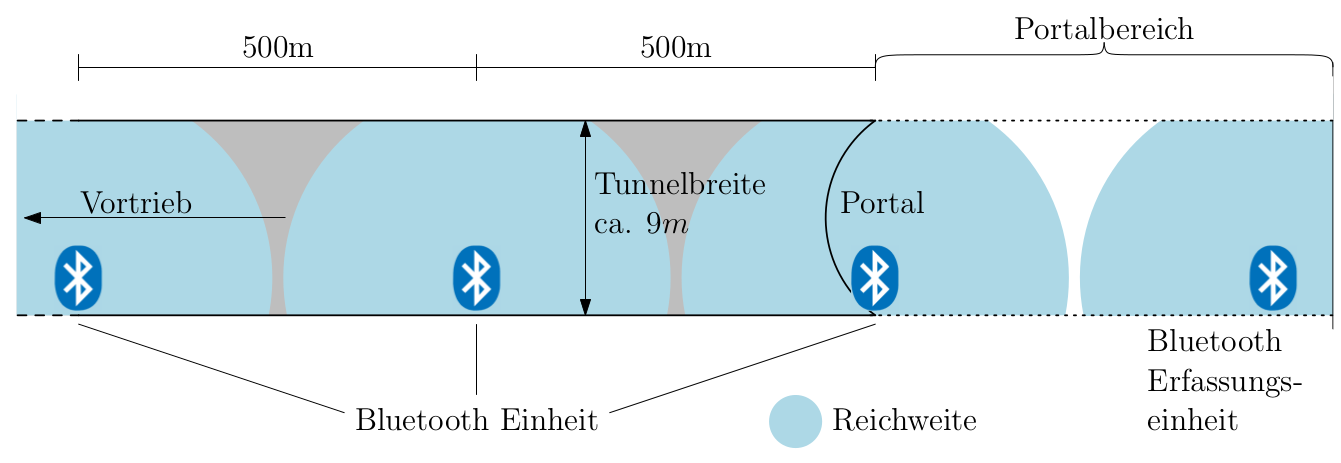
\includegraphics[width=\textwidth]{images/bisherige.png}\\
	\cite{maurer2016unterstuetzung}
\end{frame}

\begin{frame}{Zukünftige Situation}
	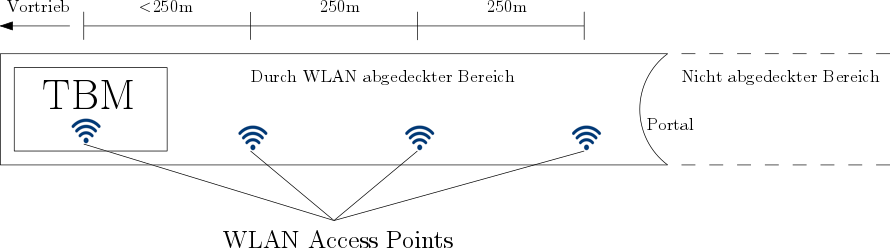
\includegraphics[width=\textwidth]{images/zukuenftige.png}
\end{frame}

\begin{frame}{Aufgabe}
	\begin{block}{Zielsetzung}
		\begin{itemize}
			\item Funkbasiertes Ortungssystem
			\item Bereichsortung (250m Abschnitte)
		\end{itemize}
	\end{block}


	\begin{block}{Anforderungen}
		\begin{itemize}
			\item Nichtintrusiv (Keine Tore, Schranken, ...)
			\item Zuverlässige Erkennung der Bereichsswechsel
			\item Wenig Interaktion mit mobiler Einheit erforderlich
		\end{itemize}
	\end{block}
\end{frame}

\section{Grundlagen \& Analyse}
\begin{frame}{Topologien}
	\begin{tabular}{c|c|c}
		\includegraphics[width=0.25\textwidth]{images/direkteselbst.eps} & \includegraphics[width=0.25\textwidth]{images/direktefern.eps} & \includegraphics[width=0.2\textwidth]{images/ohnebasis.eps}\\
		Direkte Selbstlokal. & Direkte Fernlokal. & Ohne Basisstation\\
		\hline
		\includegraphics[width=0.25\textwidth]{images/indirekteselbst.eps} & \includegraphics[width=0.25\textwidth]{images/indirektefern.eps} & \includegraphics[width=0.25\textwidth]{images/hybrid.eps} \\
	Indirekte Selbstlokal. & Indirekte Fernlokal. & Hybride Topologie\\
	\end{tabular}
\end{frame}

\begin{frame}{Fernlokalisierung}
	\begin{columns}
		\column{0.5\textwidth}
			\centering
			\includegraphics[width=\textwidth]{images/direktefern.eps}

			Direkte Fernlokalisierung

		\column{0.5\textwidth}
			\centering
			\includegraphics[width=\textwidth]{images/indirektefern.eps}

			Indirekte Fernlokalisierung
	\end{columns}
\end{frame}


\begin{frame}
	\begin{block}{Messgrößen}
		\begin{itemize}
			\item Time of Arrival
			\item Time Difference of Arrival
			\item (Roundtrip) Time of Flight
			\item Received Signal Strength (Indicator)
			\item Heartbeat
		\end{itemize}
	\end{block}

	\begin{columns}
			\column{0.5\textwidth}
				\begin{block}{Lokalisierungsprinzip}
					\begin{itemize}
						\item Umgebungsprinzip
						\item Geometrische Bestimmung
						\item Szenenanalyse
					\end{itemize}
				\end{block}

		\column{0.5\textwidth}
			\begin{block}{Protokolle}
				\begin{itemize}
					\item IEEE 802.11
					\item Bluetooth (Low Energy)
					\item Long Range (IEEE 802.15.4g)
				\end{itemize}
			\end{block}
	\end{columns}
\end{frame}


\begin{frame}{Hardware}
	\begin{tabular}{cc}
		\multicolumn{2}{c}{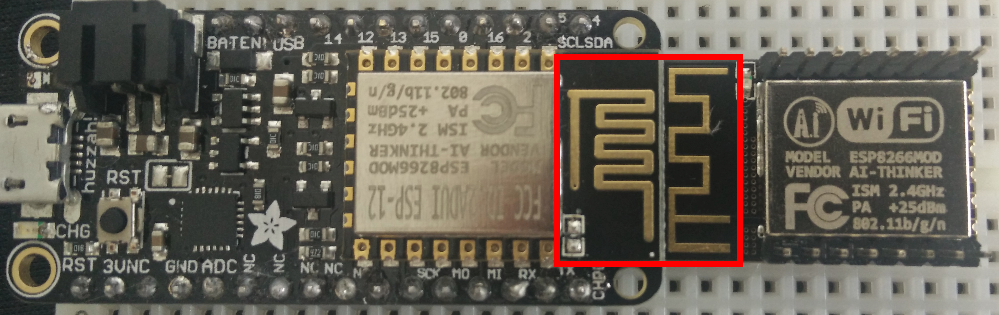
\includegraphics[width=0.9\textwidth]{images/espmodules.png}}\\
		\multicolumn{2}{c}{Adafruit Feather HUZZAH ESP8266}\\
		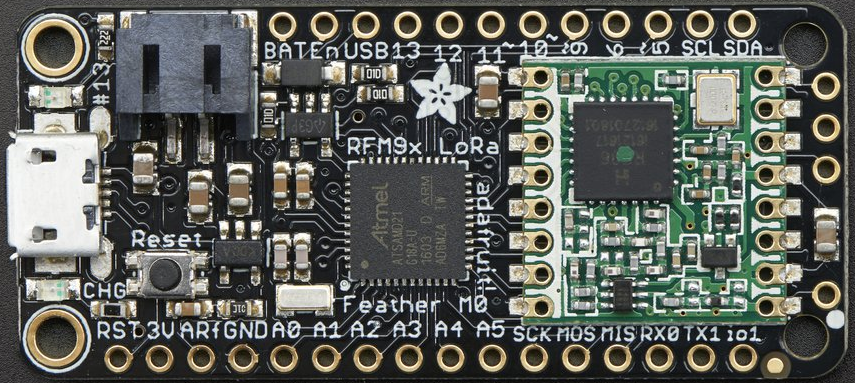
\includegraphics[width=0.45\textwidth]{images/loraada.png} & 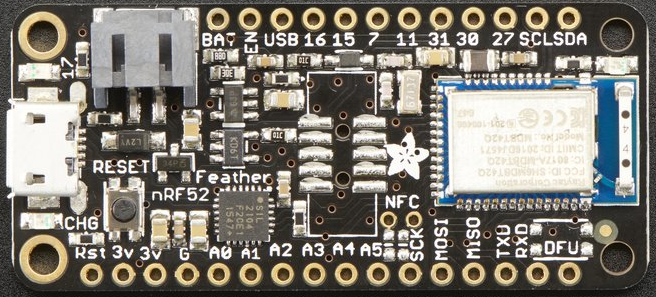
\includegraphics[width=0.45\textwidth]{images/nrf52ada.png}\\
		Feather M0 RFM95 LoRa Radio & Feather nRF52 Bluefruit\\
	\end{tabular}
\end{frame}

\section{Reichweiten}
\begin{frame}{Reichweitenevaluation - Aufbau}
	\begin{tabular}{cc}
		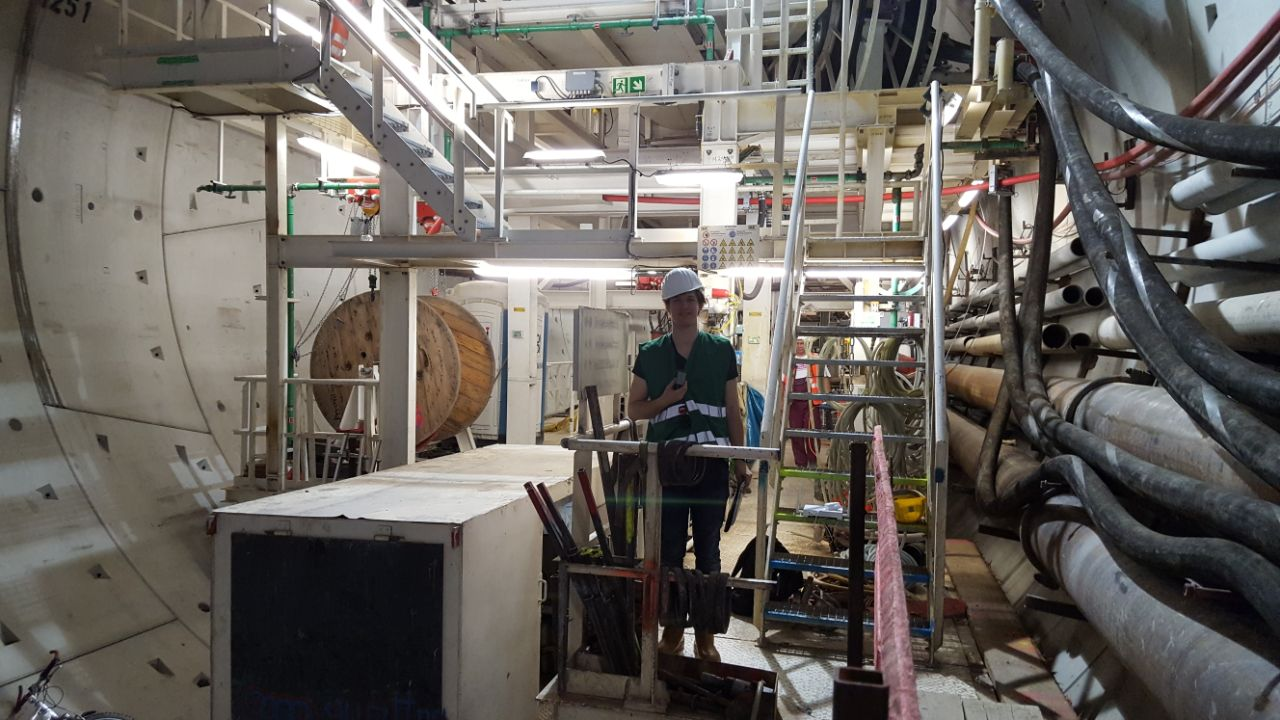
\includegraphics[width=0.45\textwidth]{images/tunnel.jpg} & 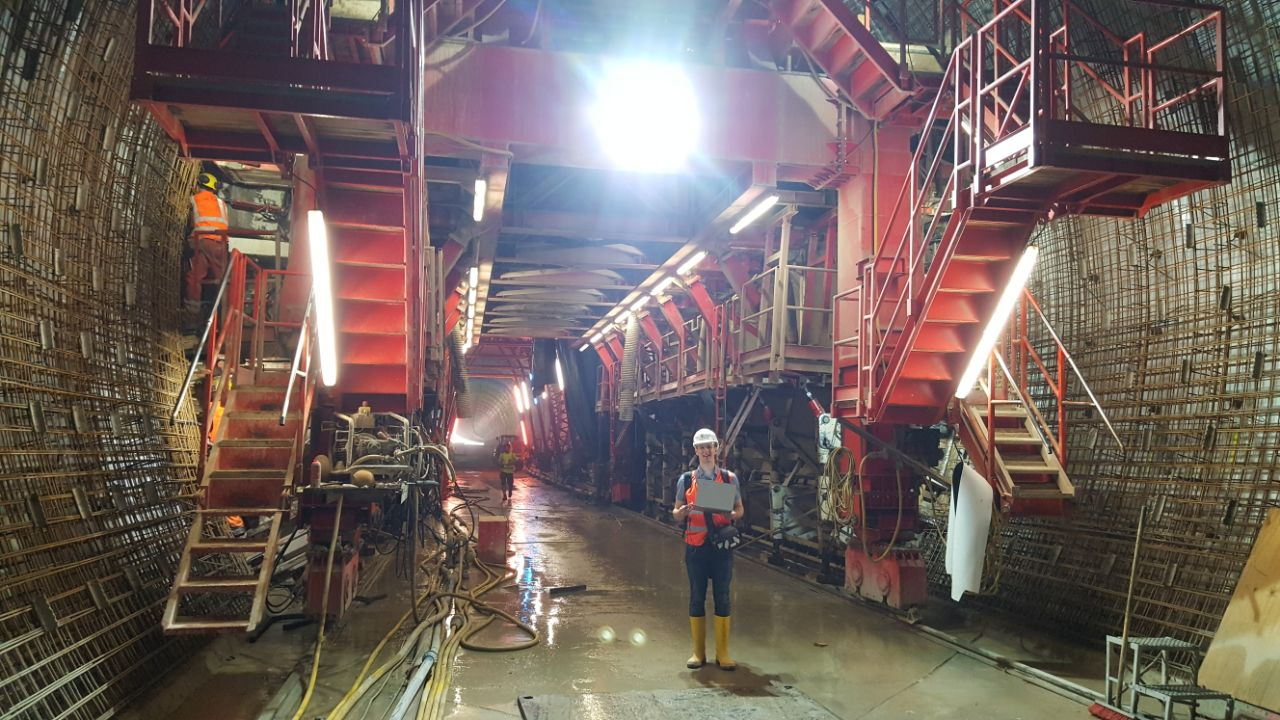
\includegraphics[width=0.45\textwidth]{images/schalungswagen.jpg}\\
		\includegraphics[width=0.45\textwidth]{images/rangewlan.eps} & \includegraphics[width=0.45\textwidth]{images/rangeblue.eps} \\
		\multicolumn{2}{c}{\includegraphics[width=0.9\textwidth]{images/rangelora.eps}}\\
	\end{tabular}
\end{frame}

\begin{frame}{Reichweitenevaluation - Ergebnisse}
	\centering
	\begin{tabular}{l|l|l}
		Protokoll & Strecke & Reichweite \\
		\hline
		BLE & Wenige Hindernisse & 32 m \\
		802.11b & Wenige Hindernisse & 88 m \\
		LoRa 5 dBm & Wenige Hindernisse & 250 m \\
		LoRa 23 dBm & Wenige Hindernisse & 1250 m \\
		\hline
		\pause
		BLE & Viele Hindernisse & 14 m \\
		802.11b & Viele Hindernisse & 32 m \\
		LoRa 5 dBm & Viele Hindernisse & 100 m \\
		LoRa 23 dBm & Viele Hindernisse & $>$350 m \\
	\end{tabular}\\
\end{frame}

\section{Implementierungen}
\subsection{RADAR}
\begin{frame}{RADAR}
	\begin{columns}
		\column{0.5\textwidth}
			\begin{block}{RADAR}
				\begin{itemize}
					\item Bahl et al. \cite{bahl2000radar}
					\item Direkte Fernlokalisierung
					\item 6 Byte mit UDP
					\item RSSI an Basisstation messen
					\item Szenenanalyse
				\end{itemize}
			\end{block}
			\centering
			\includegraphics[width=0.7\textwidth]{images/direktefern.eps}
		\column{0.5\textwidth}
			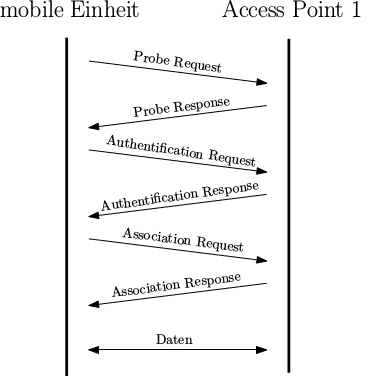
\includegraphics[width=\textwidth]{images/reupper.png}
	\end{columns}
\end{frame}

\begin{frame}{Stromverbrauch - RADAR}
	\begin{minipage}[c][\textheight][t]{\textwidth}
		\centering
		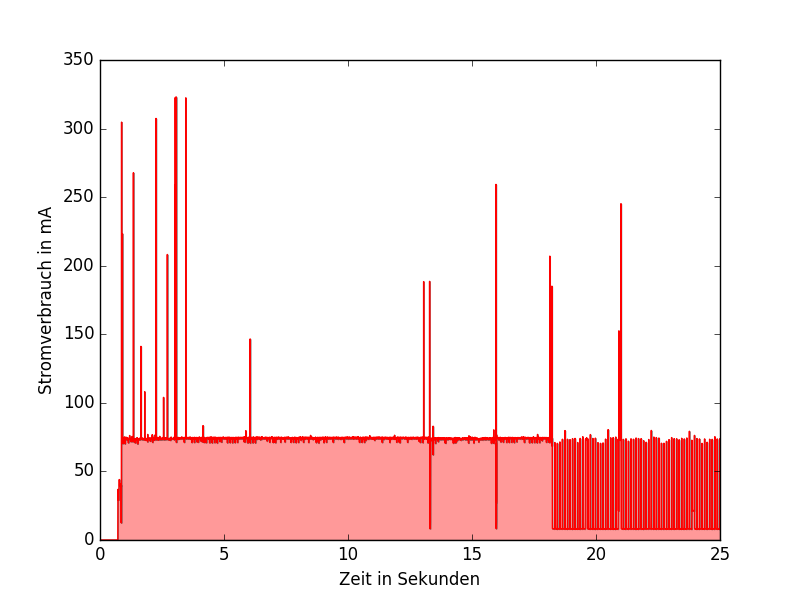
\includegraphics[height=0.85\textheight]{plots/radar5s.png}
	\end{minipage}
\end{frame}

\begin{frame}{Stromverbrauch - RADAR}
	\begin{minipage}[c][\textheight][t]{\textwidth}
		\centering
		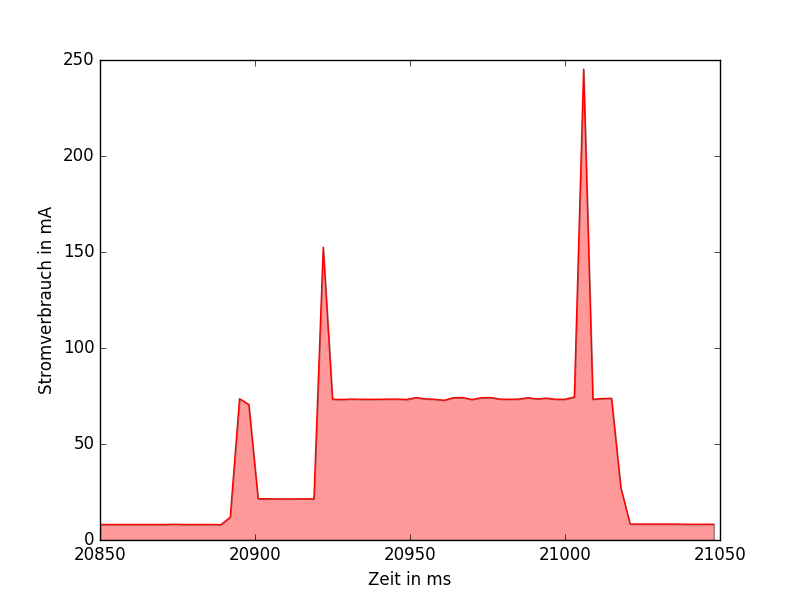
\includegraphics[height=0.85\textheight]{plots/radar5ssend.png}
	\end{minipage}
\end{frame}

\subsection{WiFi-LLS}
\begin{frame}{WiFi-LLS}
	\begin{columns}
		\column{0.5\textwidth}
			\begin{block}{WiFi-LLS}
				\begin{itemize}
					\item Chen et al. \cite{chen2007design}
					\item Indirekte Fernlokalisierung
					\item RSSI der Probe Responses
					\item An mobiler Einheit gemessen
					\item Geometrische Bestimmung
				\end{itemize}
			\end{block}
			\centering
			\includegraphics[width=0.7\textwidth]{images/indirektefern.eps}
		\column{0.5\textwidth}
			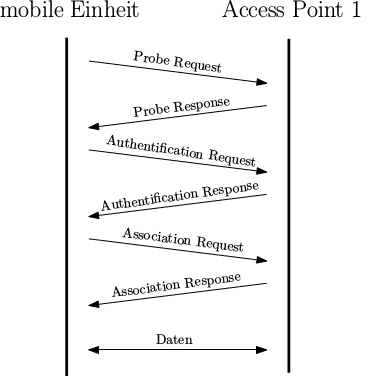
\includegraphics[width=\textwidth]{images/reupper.png}
	\end{columns}
\end{frame}

\begin{frame}{Stromverbrauch - WiFi-LLS}
	\begin{minipage}[c][\textheight][t]{\textwidth}
		\centering
		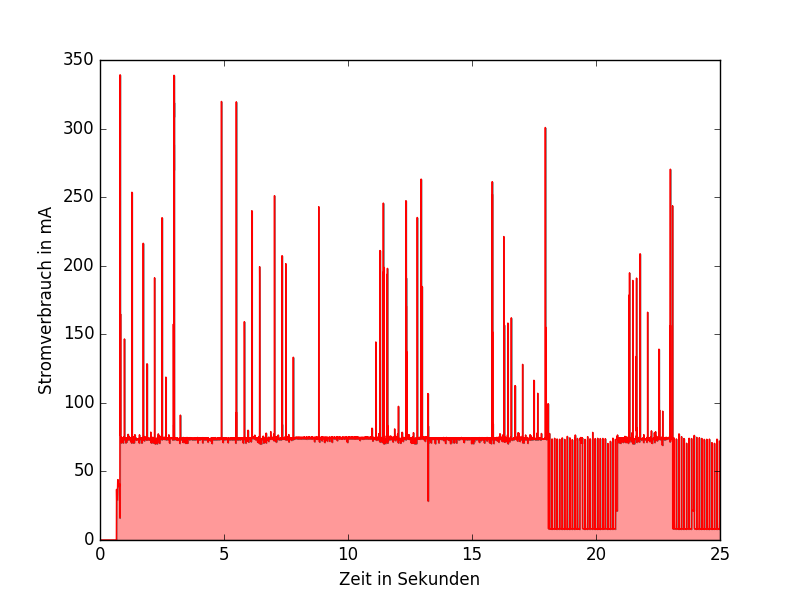
\includegraphics[height=0.85\textheight]{plots/wifills.png}
	\end{minipage}
\end{frame}

\begin{frame}{Stromverbrauch - WiFi-LLS}
	\begin{minipage}[c][\textheight][t]{\textwidth}
		\centering
		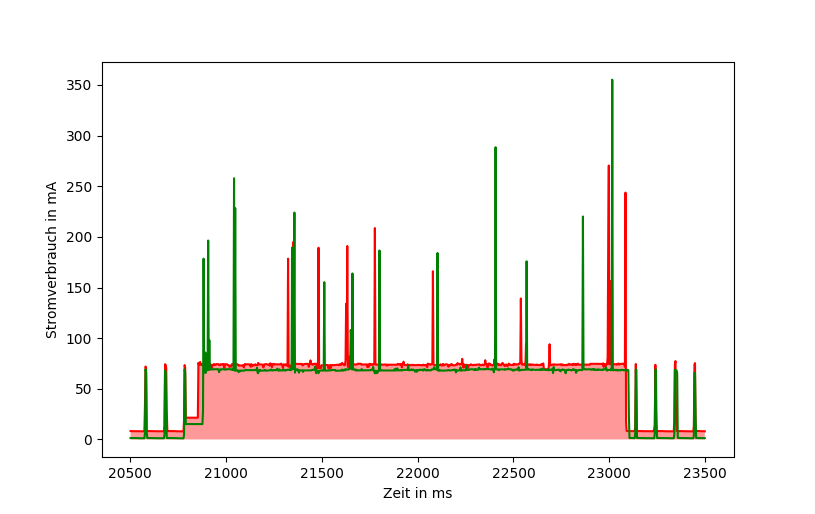
\includegraphics[height=0.85\textheight]{plots/wifillssendv.png}
	\end{minipage}
\end{frame}


\begin{frame}{Stromverbrauch - Ergebnisse}
	\begin{tabular}{l|l|l|R{2.5cm}}
		Protokoll & Modul & Programm  & $\varnothing$ Verbrauch in mA (normalisiert)\\
		\hline
		IEEE 802.11 & \emph{ESP8266} Feather & \emph{RADAR} & 16,70 (8,60)\\
		IEEE 802.11 & \emph{ESP-12F} & \emph{RADAR} & 10,10 (8,80) \\
		\hline
		IEEE 802.11 & \emph{ESP8266} Feather & \emph{WiFi-LLS} & 42,20 (34,10)\\
		IEEE 802.11 & \emph{ESP-12F} & \emph{WiFi-LLS} & 36,50 (35,20)\\
	\end{tabular}
\end{frame}

\subsection{Assoziations-Lokalisierung}
\begin{frame}{Assoziations-Lokalisierung}
	\begin{tabular}{cc}
		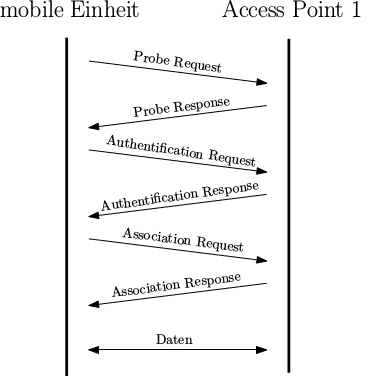
\includegraphics[height=0.5\textheight]{images/reupper.png} & 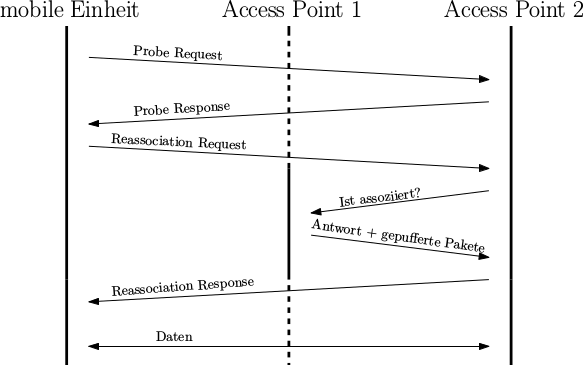
\includegraphics[height=0.5\textheight]{images/relower.png}\\
	\end{tabular}
	\begin{block}{Assoziations-Lokalisierung}
		\begin{itemize}
			\item Indirekte Fernlokalisierung
			\item Erfolgreiche (Re-)Assoziation, implizit RSSI der Probe Responses
			\item Umgebungsprinzip
			\item Für Bereichsortung geeignet
		\end{itemize}
	\end{block}
\end{frame}

\begin{frame}{Stromverbrauch - Assoziations-Lok.}
	\begin{minipage}[c][\textheight][t]{\textwidth}
		\centering
		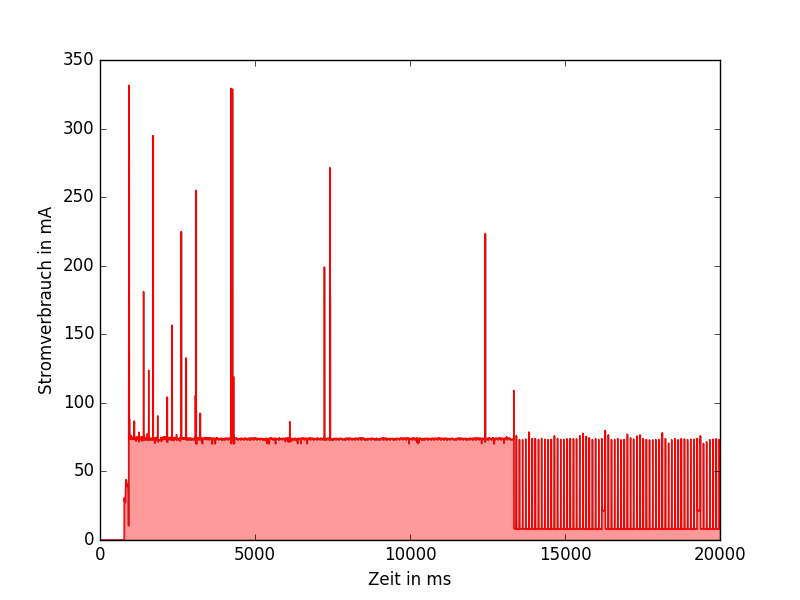
\includegraphics[height=0.85\textheight]{plots/tcphold.png}
	\end{minipage}
\end{frame}

\begin{frame}{Stromverbrauch - Assoziations-Lok.}
	\begin{minipage}[c][\textheight][t]{\textwidth}
		\centering
		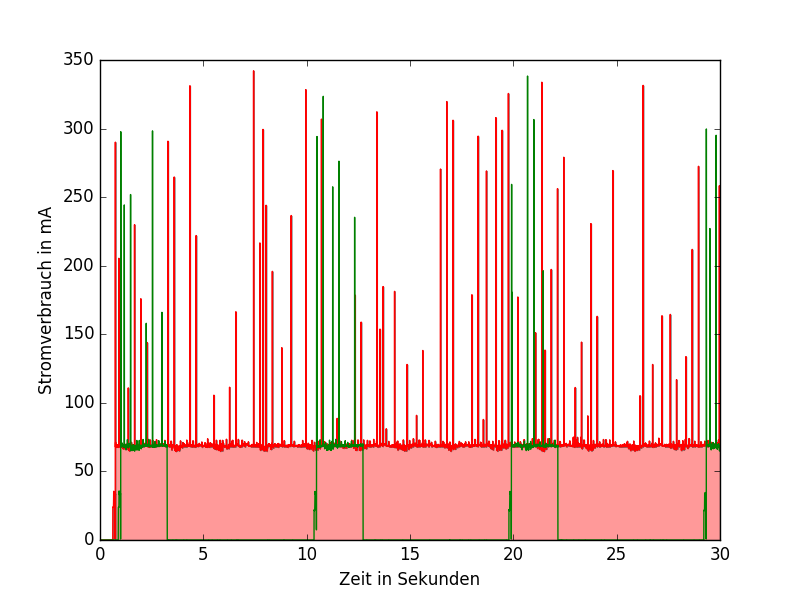
\includegraphics[height=0.85\textheight]{plots/noap.png}
	\end{minipage}
\end{frame}

\begin{frame}{Stromverbrauch - Ergebnisse}
	\begin{tabular}{l|l|p{3.1cm}|R{2.1cm}}
		Protokoll & Modul & Programm  & $\varnothing$ Verbrauch in mA (normalisiert)\\
		\hline
		IEEE 802.11 & \emph{ESP8266} Feather & \emph{RADAR} & 16,70 (8,60)\\
		IEEE 802.11 & \emph{ESP-12F} & \emph{RADAR} & 10,10 (8,80) \\
		\hline
		IEEE 802.11 & \emph{ESP8266} Feather & \emph{WiFi-LLS} & 42,20 (34,10)\\
		IEEE 802.11 & \emph{ESP-12F} & \emph{WiFi-LLS} & 36,50 (35,20)\\
		\hline
		IEEE 802.11 & \emph{ESP-12F} & \emph{Assoziations-Lokalisierung} & 8,80 (7,50)\\
		IEEE 802.11 & \emph{ESP-12F} & \emph{Assoziations-Lokalisierung} (kein \emph{Access Point}) & 17,10 (17,10)\\
	\end{tabular}
\end{frame}

\subsection{Probe-Request-Lokalisierung}
\begin{frame}{Probe-Request-Lokalisierung}
	\begin{columns}
		\column{0.5\textwidth}
			\begin{block}{Probe-Request-Lokalisierung}
				\begin{itemize}
					\item Direkte Fernlokalisierung
					\item RSSI der Probe Requests
					\item An Access Point gemessen
					\item Umgebungsprinzip
				\end{itemize}
			\end{block}
			\centering
			\includegraphics[width=0.7\textwidth]{images/direktefern.eps}
		\column{0.5\textwidth}
			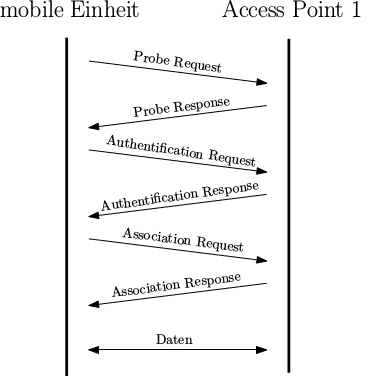
\includegraphics[width=\textwidth]{images/reupper.png}
	\end{columns}
\end{frame}

\begin{frame}{Stromverbrauch - Probe-Request-Lok.}
	\begin{minipage}[c][\textheight][t]{\textwidth}
		\centering
		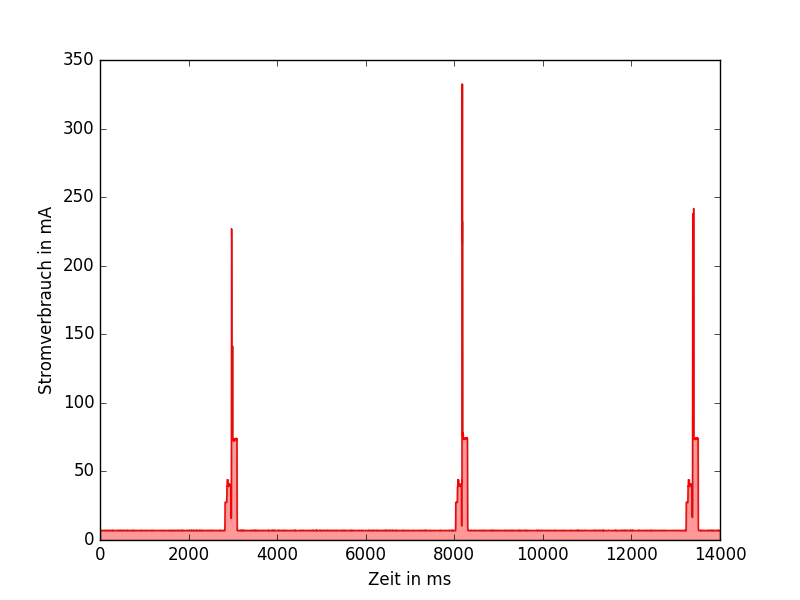
\includegraphics[height=0.85\textheight]{plots/probereqfull.png}
	\end{minipage}
\end{frame}

\begin{frame}{Stromverbrauch - Probe-Request-Lok.}
	\begin{minipage}[c][\textheight][t]{\textwidth}
		\centering
		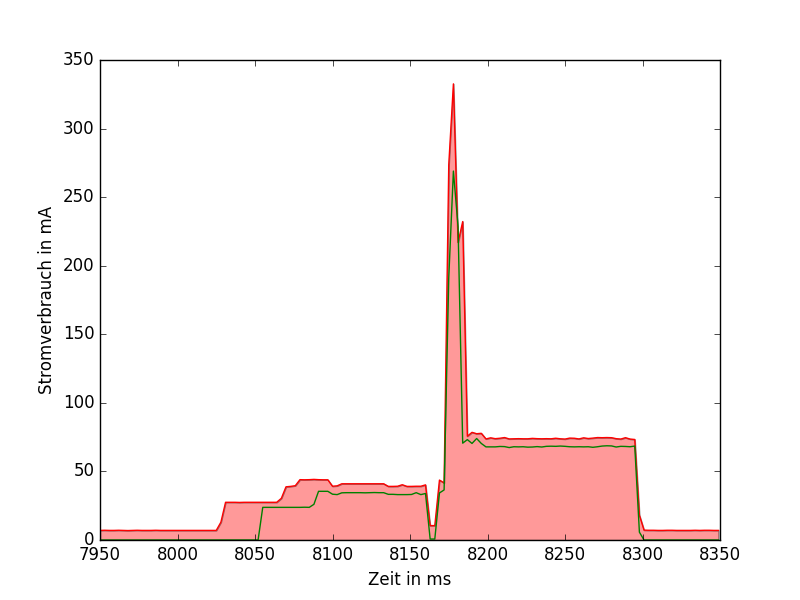
\includegraphics[height=0.85\textheight]{plots/probereqv.png}
	\end{minipage}
\end{frame}

\begin{frame}{Stromverbrauch - Ergebnisse}
	\begin{tabular}{l|l|p{3.1cm}|R{2.1cm}}
		Protokoll & Modul & Programm  & $\varnothing$ Verbrauch in mA (normalisiert)\\
		\hline
		IEEE 802.11 & \emph{ESP-12F} & \emph{Assoziations-Lokalisierung} & 8,80 (7,50)\\
		IEEE 802.11 & \emph{ESP-12F} & \emph{Assoziations-Lokalisierung} (kein \emph{Access Point}) & 17,10 (17,10)\\
		\hline
		IEEE 802.11 & \emph{ESP8266} Feather & \emph{Probe-Request-Lokalisierung} & 9,70 (2,70)\\
		IEEE 802.11 & \emph{ESP-12F} & \emph{Probe-Request-Lokalisierung} & 1,80 (1,80)\\
		\hline
	\end{tabular}
\end{frame}


\subsection{Bluetooth Low Energy}
\begin{frame}{Bluetooth Low Energy}
	\begin{columns}
		\column{0.5\textwidth}
			\begin{block}{BLE-Advertising}
				\begin{itemize}
					\item Jianyong et al. \cite{jianyong2014rssi}
					\item Direkte Fernlokalisierung
					\item RSSI von Advertising Paketen
					\item An Basisstation gemessen
					\item Umgebungsprinzip
				\end{itemize}
			\end{block}
		\column{0.5\textwidth}
			\centering
			\includegraphics[width=\textwidth]{images/direktefern.eps}
	\end{columns}
\end{frame}

\begin{frame}{Stromverbrauch - BLE-Advertising}
	\begin{minipage}[c][\textheight][t]{\textwidth}
		\centering
		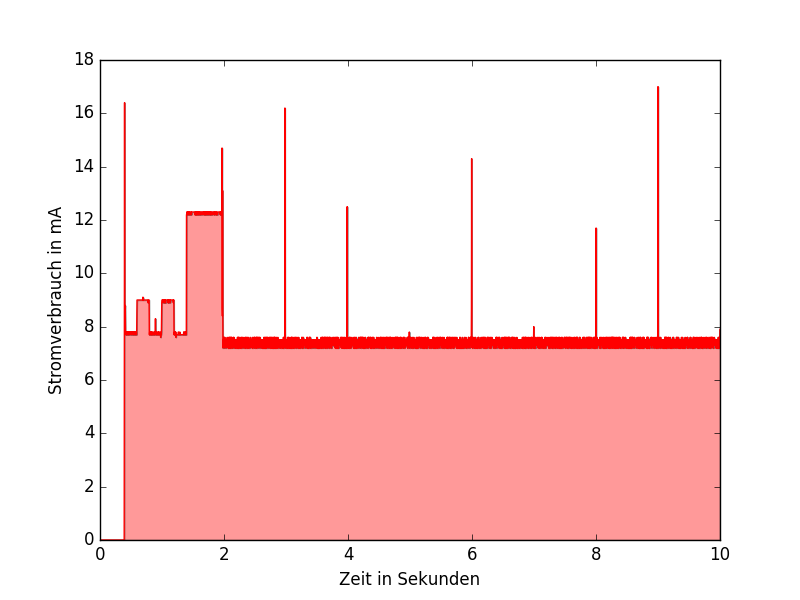
\includegraphics[height=0.85\textheight]{plots/blue.png}
	\end{minipage}
\end{frame}

\begin{frame}{Stromverbrauch - Ergebnisse}
	\begin{tabular}{l|l|p{3.1cm}|R{2.1cm}}
		Protokoll & Modul & Programm  & $\varnothing$ Verbrauch in mA (normalisiert)\\
		\hline
		IEEE 802.11 & \emph{ESP8266} Feather & \emph{Probe-Request-Lokalisierung} & 9,70 (2,70)\\
		IEEE 802.11 & \emph{ESP-12F} & \emph{Probe-Request-Lokalisierung} & 1,80 (1,80)\\
		\hline
		BLE & \emph{nRF52} Feather & Ortung mit \emph{BLE-Advertising} & 7,37 (0,04)\\
	\end{tabular}
\end{frame}

\subsection{Lokalisierung mit LoRa}
\begin{frame}{Lokalisierung mit LoRa}
	\begin{columns}
		\column{0.5\textwidth}
			\begin{block}{Lokalisierung mit LoRa}
				\begin{itemize}
					\item Direkte Fernlokalisierung
					\item RSSI an Basisstation gemessen
					\item Geometrische Bestimmung
				\end{itemize}
			\end{block}
		\column{0.5\textwidth}
			\centering
			\includegraphics[width=\textwidth]{images/direktefern.eps}
	\end{columns}
\end{frame}

\begin{frame}{Stromverbrauch - LoRa}
	\begin{minipage}[c][\textheight][t]{\textwidth}
		\centering
		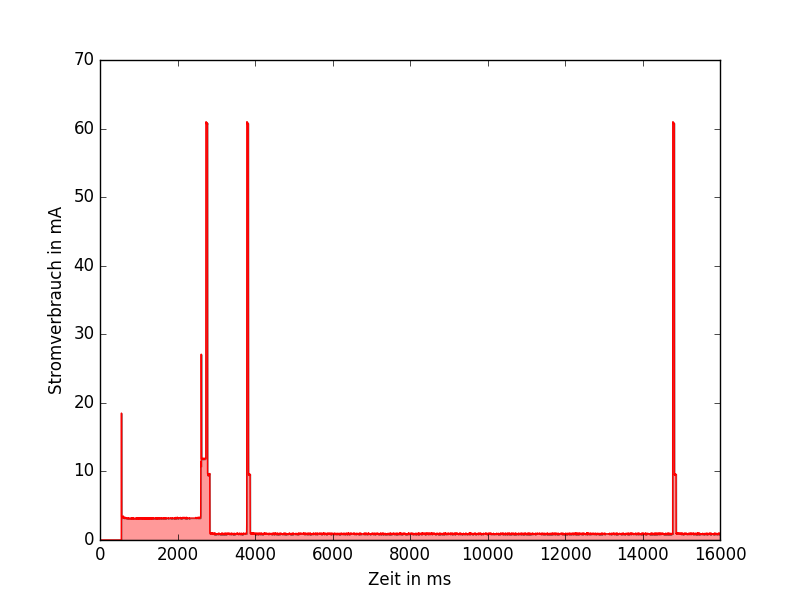
\includegraphics[height=0.85\textheight]{plots/lora5.png}
	\end{minipage}
\end{frame}

\begin{frame}{Stromverbrauch - LoRa}
	\begin{minipage}[c][\textheight][t]{\textwidth}
		\centering
		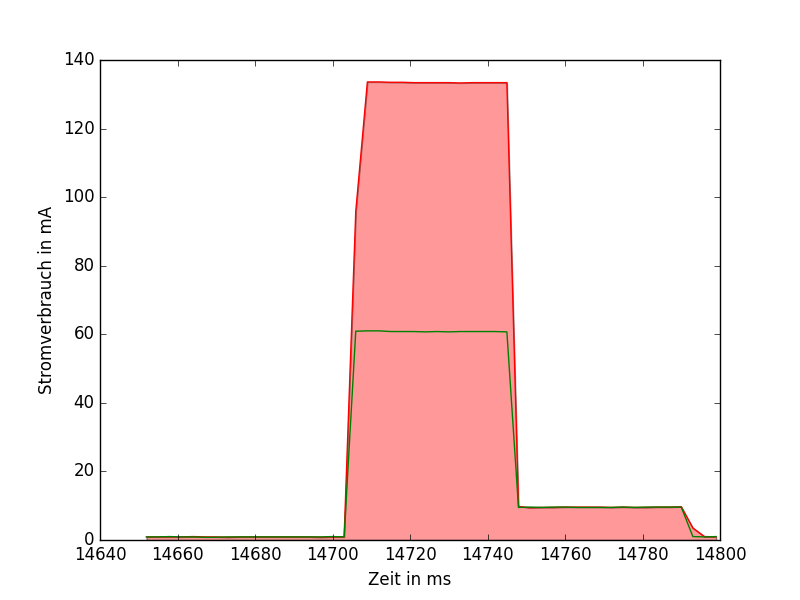
\includegraphics[height=0.85\textheight]{plots/lora235send.png}
	\end{minipage}
\end{frame}

\begin{frame}{Stromverbrauch - Ergebnisse}
	\begin{tabular}{l|p{3cm}|p{3cm}|R{2.1cm}}
		Protokoll & Modul & Programm  & $\varnothing$ Verbrauch in mA (normalisiert)\\
		\hline
		IEEE 802.11 & \emph{ESP-12F} & \emph{Probe-Request-Lokalisierung} & 1,80 (1,80)\\
		\hline
		BLE & \emph{nRF52} Feather & Ortung mit \emph{BLE-Advertising} & 7,37 (0,04)\\
		\hline
		LoRa & \emph{RFM95} Feather 5 dBM & Ortung mit LoRa RSSI & 1,20 (0,30)\\
		LoRa & \emph{RFM95} Feather 23 dBM & Ortung mit LoRa RSSI & 1,47 (0,57)\\
	\end{tabular}
\end{frame}

\section{Zusammenfassung}
\begin{frame}{Stromverbrauch - Vergleich}
	\begin{minipage}[c][\textheight][t]{\textwidth}
		\centering
		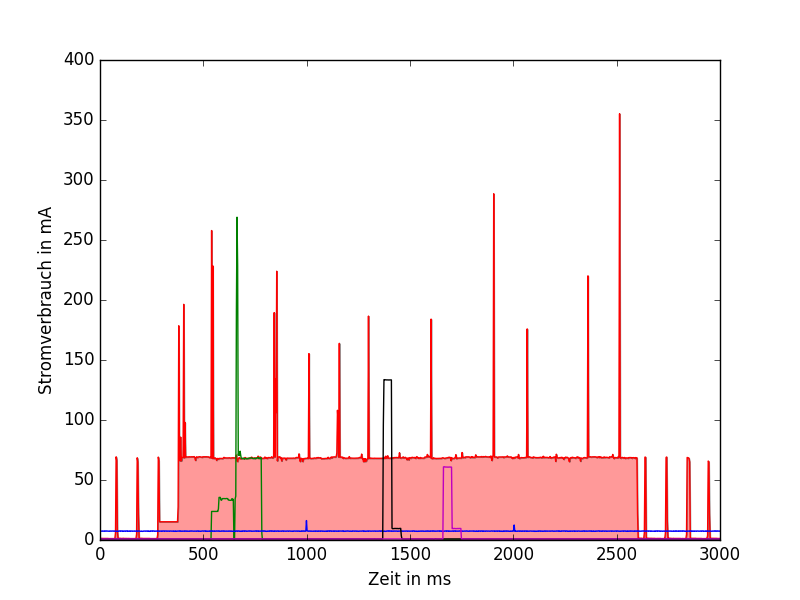
\includegraphics[height=0.85\textheight]{plots/alle.png}
	\end{minipage}
\end{frame}

\begin{frame}{Stromverbrauch - Vergleich}
	\begin{minipage}[c][\textheight][t]{\textwidth}
		\centering
		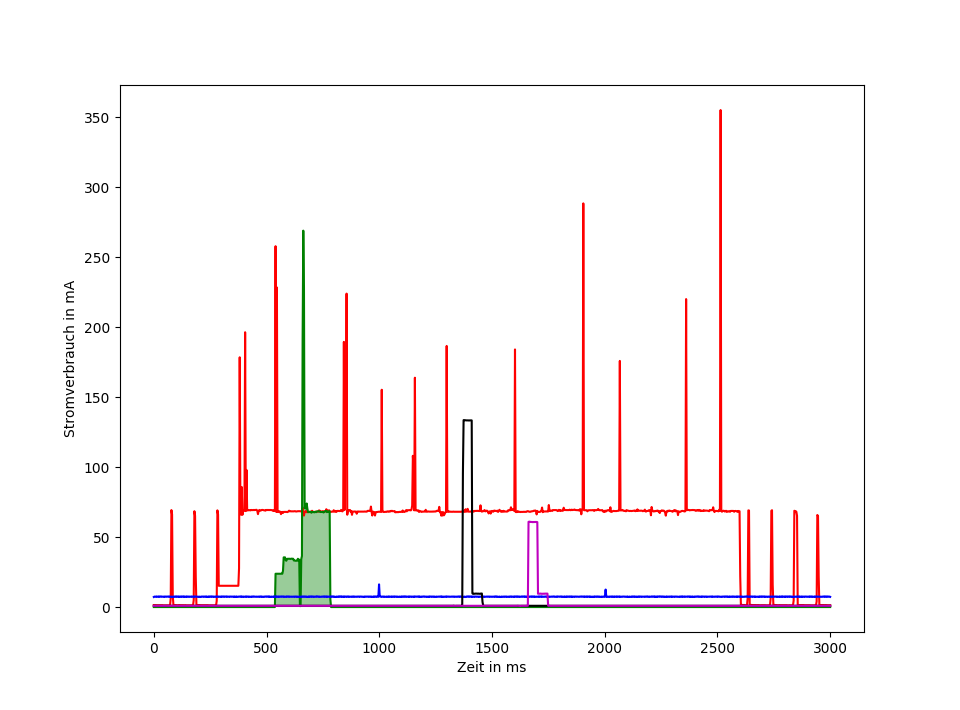
\includegraphics[height=0.85\textheight]{plots/alle2.png}
	\end{minipage}
\end{frame}

\begin{frame}{Stromverbrauch - Vergleich}
	\begin{minipage}[c][\textheight][t]{\textwidth}
		\centering
		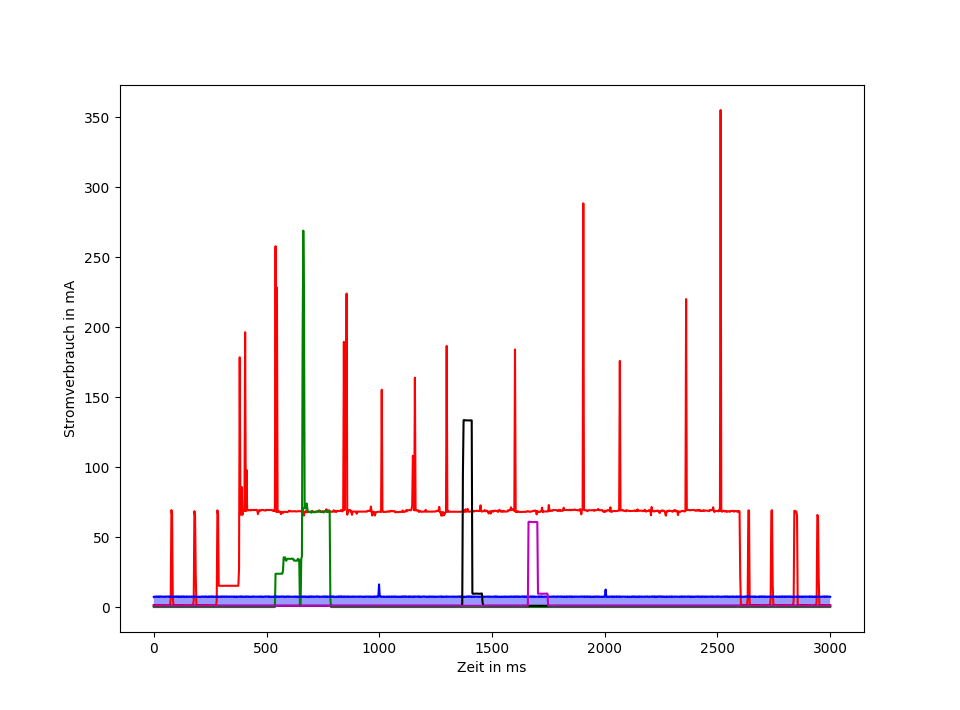
\includegraphics[height=0.85\textheight]{plots/alle3.png}
	\end{minipage}
\end{frame}

\begin{frame}{Stromverbrauch - Vergleich}
	\begin{minipage}[c][\textheight][t]{\textwidth}
		\centering
		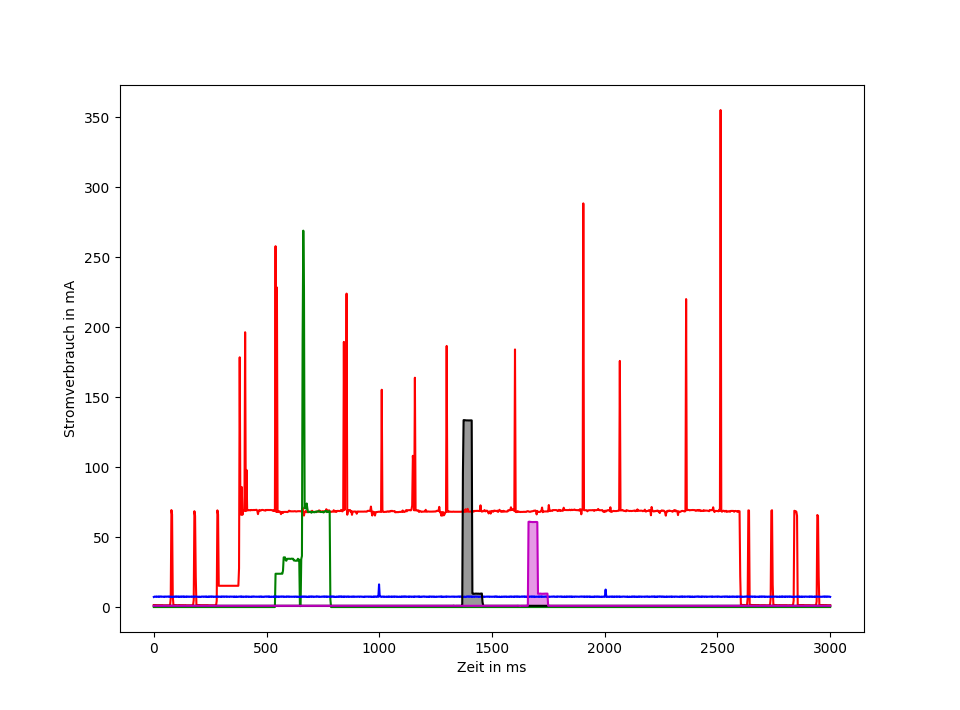
\includegraphics[height=0.85\textheight]{plots/alle4.png}
	\end{minipage}
\end{frame}

\begin{frame}{Stromverbrauch - Ergebnisse}
	\begin{tabular}{l|p{3cm}|p{3.1cm}|R{2.1cm}}
		Protokoll & Modul & Programm  & $\varnothing$ Verbrauch in mA (normalisiert)\\
		\hline
		IEEE 802.11 & \emph{ESP-12F} & \emph{RADAR} & 10,10 (8,80) \\
		\hline
		IEEE 802.11 & \emph{ESP-12F} & \emph{WiFi-LLS} & 36,50 (35,20)\\
		\hline
		IEEE 802.11 & \emph{ESP-12F} & \emph{Assoziations-Lokalisierung} & 8,80 (7,50)\\
		IEEE 802.11 & \emph{ESP-12F} & \emph{Assoziations-Lokalisierung} (kein \emph{Access Point}) & 17,10 (17,10)\\
		\hline
		IEEE 802.11 & \emph{ESP-12F} & \emph{Probe-Request-Lokalisierung} & 1,80 (1,80)\\
		\hline
		BLE & \emph{nRF52} Feather & Ortung mit \emph{BLE-Advertising} & 7,37 (0,04)\\
		\hline
		LoRa & \emph{RFM95} Feather 5 dBM & Ortung mit LoRa RSSI & 1,20 (0,30)\\
		LoRa & \emph{RFM95} Feather 23 dBM & Ortung mit LoRa RSSI & 1,47 (0,57)\\
	\end{tabular}
\end{frame}

\section{Fazit}
\begin{frame}{Fazit}
	\begin{minipage}[t][0.5\textheight][t]{\textwidth}
		\centering
		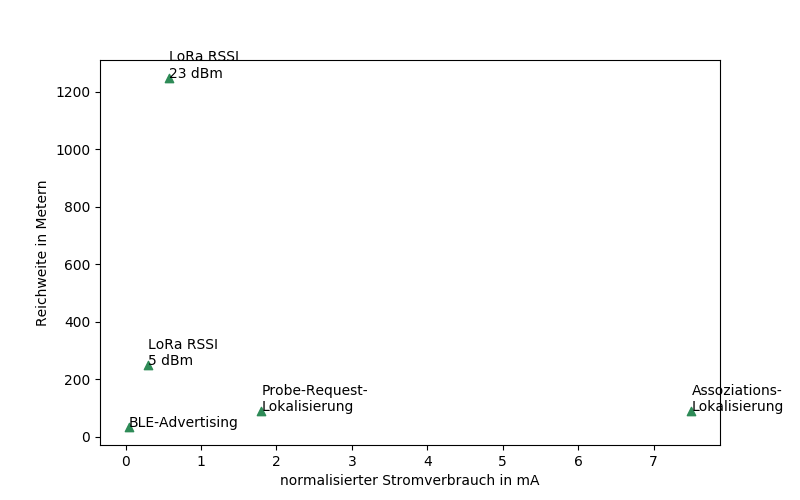
\includegraphics[width=0.9\textheight]{plots/scatterplot.png}
	\end{minipage}


	\begin{block}{Konklusion}
			\begin{itemize}
				\item LoRa > 802.11
				\item LoRa ohne Erfassungslücken => Hohe Zuverlässigkeit
				\item BLE hat niedrigen Stromverbrauch => Wenig Interaktion notwendig
			\end{itemize}
	\end{block}

\end{frame}


\appendix
\beginbackup

\begin{frame}[allowframebreaks]{References}
\printbibliography
\end{frame}

\begin{frame}{ESP8266 Verbrauch}%Verbrauch ESP
	\begin{minipage}[t][\textheight][t]{\textwidth}
		\centering
		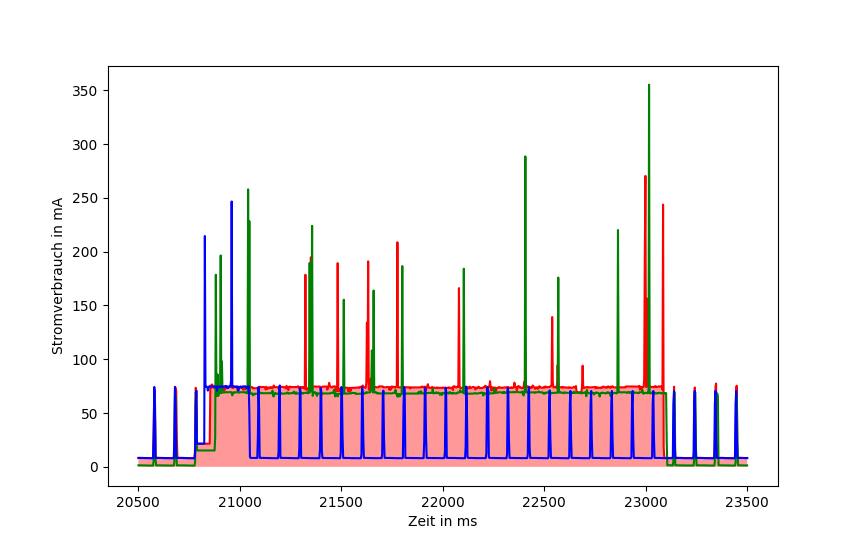
\includegraphics[width=0.95\textwidth]{plots/wifillssendv2.png}
	\end{minipage}
\end{frame}

\begin{frame}{TDOA}%TDOA
	\begin{minipage}[t][0.8\textheight][t]{\textwidth}
		\centering
		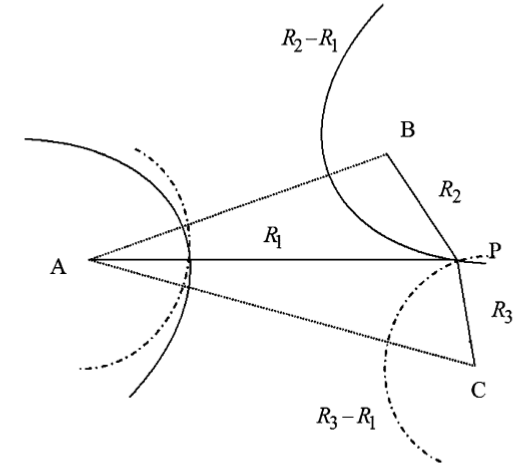
\includegraphics[height=0.6\textheight]{images/tdoa.png}\\
		$R_{i,j} = \sqrt{(x_i - x)^2 + (y_i - y)^2 + (z_i - z)^2} - \sqrt{(x_j - x)^2 + (y_j - y)^2 + (z_j - z)^2}$
	\end{minipage}
\end{frame}

\begin{frame}{Inquiry Scan}%Inquiry Scan
	\begin{minipage}[t][\textheight][t]{\textwidth}
		\centering
		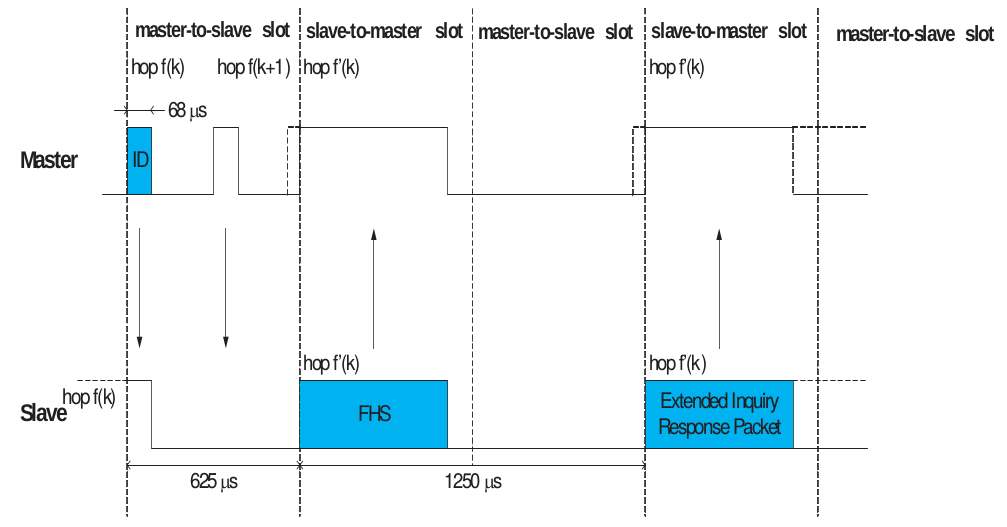
\includegraphics[width=0.95\textwidth]{images/inqscan.png}
	\end{minipage}
\end{frame}

\begin{frame}{IEEE 802.11 RSSI}%RSSI 802.11
	\begin{minipage}[t][\textheight][t]{\textwidth}
		\centering
		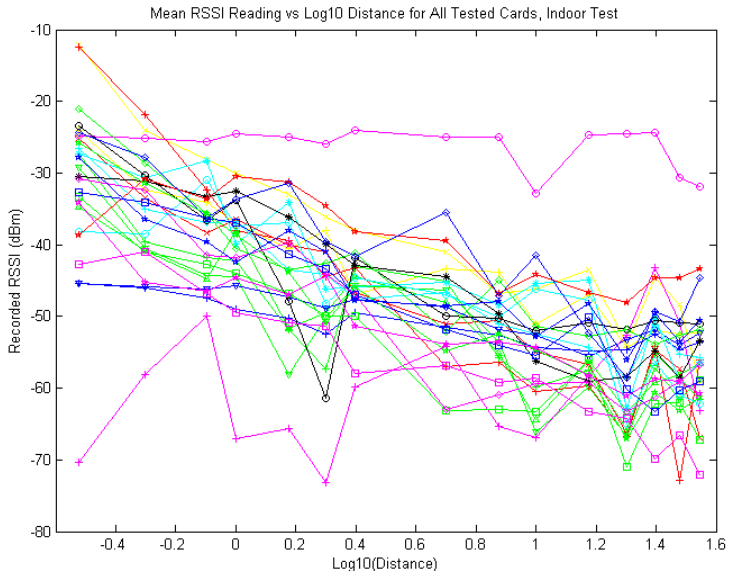
\includegraphics[height=0.8\textheight]{images/luiRSSI.png}
	\end{minipage}
\end{frame}

\begin{frame}{Bluetooth Messgrößen}%Bluetooth Messwerte
	\begin{minipage}[t][\textheight][t]{\textwidth}
		\centering
		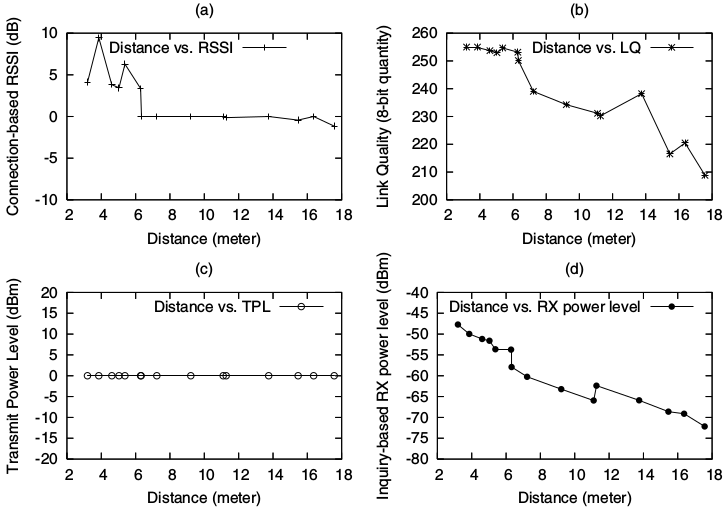
\includegraphics[height=0.8\textheight]{images/bluetoothmess.png}
	\end{minipage}
\end{frame}

\begin{frame}{ESP8266 Verbrauch}%Verbrauch ESP
	\begin{minipage}[t][\textheight][t]{\textwidth}
		\centering
		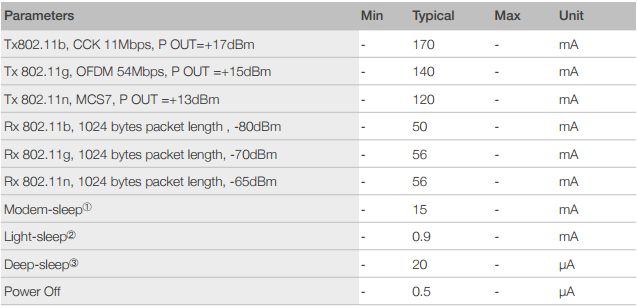
\includegraphics[width=0.95\textwidth]{images/esppower.png}
	\end{minipage}
\end{frame}

\begin{frame}{nRF52 Verbrauch}%Verbrauch nRF52
	\begin{minipage}[t][\textheight][t]{\textwidth}
		\centering
		\includegraphics[width=0.9\textwidth]{images/nrf52consumption.png}
	\end{minipage}
\end{frame}

\begin{frame}{M0/RFM95 Verbrauch}%Verbrauch M0/RFM95
	\begin{minipage}[t][\textheight][t]{\textwidth}
		\centering
		\includegraphics[height=0.4\textheight]{images/m0power.png}\\
		\includegraphics[height=0.4\textheight]{images/lorapower.png}
	\end{minipage}
\end{frame}

\backupend

\end{document}
